%%% Template from: https://www.sharelatex.com/templates/thesis/thesis-template-with-memoir

\documentclass[11pt,a4paper]{memoir}
\usepackage[dvips]{graphicx}
\usepackage{xcolor}
\usepackage{float}
\usepackage[backend=bibtex]{biblatex}
\usepackage{caption}
\usepackage{subcaption}
\usepackage{wasysym}
\usepackage[printonlyused]{acronym}

\usepackage[
breaklinks=true,colorlinks=true,
%linkcolor=blue,urlcolor=blue,citecolor=blue,% PDF VIEW
linkcolor=black,urlcolor=black,citecolor=black,% PRINT
bookmarks=true,bookmarksopenlevel=2]{hyperref}

\usepackage{geometry}
\graphicspath{ {Figures/} }


% PDF VIEW
% \geometry{total={210mm,297mm},
% left=25mm,right=25mm,%
% bindingoffset=0mm, top=25mm,bottom=25mm}
% PRINT
\geometry{total={210mm,297mm},
left=20mm,right=20mm,
bindingoffset=10mm, top=25mm,bottom=25mm}

\OnehalfSpacing
%\linespread{1.3}

%%% CHAPTER'S STYLE
\chapterstyle{bianchi}
%\chapterstyle{ger}
%\chapterstyle{madsen}
%\chapterstyle{ell}
%%% STYLE OF SECTIONS, SUBSECTIONS, AND SUBSUBSECTIONS
\setsecheadstyle{\Large\bfseries\sffamily\raggedright}
\setsubsecheadstyle{\large\bfseries\sffamily\raggedright}
\setsubsubsecheadstyle{\bfseries\sffamily\raggedright}


%%% STYLE OF PAGES NUMBERING
%\pagestyle{companion}\nouppercaseheads 
%\pagestyle{headings}
%\pagestyle{Ruled}
\pagestyle{plain}
\makepagestyle{plain}
\makeevenfoot{plain}{\thepage}{}{}
\makeoddfoot{plain}{}{}{\thepage}
\makeevenhead{plain}{}{}{}

\bibliography{references}

\author{Joseph Redfern}
\title{Video to audio conversion for visually impaired}
\date{}

\begin{document}

\thispagestyle{empty}

{%%%
\sffamily
\centering
\Large

~\vspace{\fill}

{\huge 
    Video to Audio converstion for the Visually Impared
}

\vspace{2.5cm}

{\LARGE
    Joseph Redfern
}

\vspace{3.5cm}

School of Computer Science \& Informatics\\
Cardiff University

\vspace{3.5cm}

Supervisor: Dr Kirill Sidorov 

\vspace{\fill}

May 2015

}

\cleardoublepage

\begin{abstract}
    This final year project report details possible methods of sonfifying video and depth data, with the view to allowing a blind person to navigate a room without any additional assistance.

    The report also details and critically evaluates existing solutions to the problem of video to audio conversion, noting their shortcomings and pointing out areas in which they are successful. 

    By means of an experimental approach, several prototype systems are explained and discussed. Relevant theory has been explained where deemed necessary --- including concepts relating to image segmentation, descriptor extraction, shape classification and tone generation.
\end{abstract}


\clearpage

\tableofcontents*

\clearpage

\chapter{Introduction}
\ac{WHO} figures claim that as as of 2012, there are 285 million people suffering from visual imparements~\cite{whoblindness}, 30 million of whom are blind. The \ac{WHO} also state that 90\% of the visually impared live in developing countries. Combined with statistics from the guide dogs for the blind association, who claim that the life-time cost of training and keeping a guide dog is around £50,000, a sad picture is painted the majority who are unable to afford visual aids.

\section{Aims and Goals}
This project aims to research and develop a methods of conveying visual information without the user of the system requiring a functional visual system. The study investigates both navigational and semantic modes of operation, and the different techniques associated with each implementation.

The goal of the project is to provide a functional system, able to be used to effectivley navigate around a room and avoid obstacles without the use of eyes.  

\section{Intended Audience}
The main intended audience for this project is the visually impared. It is anticipated that the "tech savvy" visually impared would be interested in trialling the prototypes, both for day-to-day use, and to assist in further development.

The system does not (initially) intend to replace all other forms of visual assistance - rather, it intends to assist those who are unable to afford luxuries such as Guide-dogs or Guide-horses~\cite{guidehorse}. A low-cost system that is capable of assisting a user in navigating a room and detecting obsticles has the potential to be life changing - even if only a small fraction of a normal, functional visual system can be imitated, 0.01\% is infinitley greater than 0.00\%.

\section{Project Scope}
The project has a fairly broad scope, and includes:
\begin{enumerate}
    \item Image Segmentation \hfill \\
    This deals with the extracting the input image, and extracting an object of interest
    \item Descriptor Extraction \hfill \\
    This is the extraction of descriptors from the object of interest (obtained from step 1)
    \item Descriptor Sonification \hfill \\
    Sonification of the output from step 2.
\end{enumerate}

Components/considerations \textbf{outside} of the scope of this project are:

\begin{enumerate}
    \item Ethical Considerations \hfill \\
    Medical Trials/patient interviews are currently outside of scope of the project, and could be considered at a later date.
    \item Robust Testing \hfill \\
\end{enumerate}



\chapter{Background}
\section{Problem Context}
\subsection{UK Statistics}
In the UK alone, around 2,000,000 people live with sight loss --- around 360,000 of which are registered with their local authority as being blind or visually impaired, who have severe and irreversible sight loss~\cite{uk-blind}.  Of these 360,000 people, there are only 17,000 white cane-users, and less than 4,800~\cite{guidedog-count} guide-dog owners. Assuming no overlap between guide dog users and white cane users, this leaves almost 94\% without access to the two major forms of assistance available to the blind. It has been estimated that the economic cost of blindness to the UK alone be in the region of \pounds22 billion~\cite{blindcost}.

A possible factor that could explain the relatively small adoption of Guide Dogs is their cost --- as mentioned in section \ref{chap:introduction}, the life-time cost of a guide dog is around \pounds50,000. Although the dog is paid for in its entirety by the Guide Dogs for the Blind association, they themselves are a charity and do not receive government funding. A system whereby the visually impaired could purchase a guide-dog would likely not be effective, as 66\% of the registered blind/partially sighted are not in paid employment~\cite{afbff} so would be unlikely to be able to afford the cost.

\subsection{Developing Countries}
The situation in less developed countries than the UK is far worse. According to the Himalayan Cataract Project~\cite{worldblindness}, ``blindness is most prevalent in developing countries where malnutrition, inadequate health and education services, poor water quality and a lack of sanitation leads to a high incidence of eye disease''. If these countries are so impoverished that they are unable to afford services that are considered basic human rights in the developed world, it is unlikely that they will be able to afford to spend \pounds50,000 per person on guide dogs. 

Although white canes are a cheaper, they are not without their downsides. They have limited range --- typically a few feet in-front of the user. This makes finding doorways etc a more difficult task than when using a guide-dog.

\section{The Problem}
This project aims to address the lack of a cheap, intuitive way of enhancing the mobility of the visually impaired. It is non-trivial to convey visual information in the form of audio, for a number of reasons.

\subsection{Compression}
\label{sec:compression}
Measuring the bit-rate of sensory systems is not an easy task~--- however, research has been done into the informational capacity of both the human visual system, and human auditory system.

Evidence makes it clear that the human visual system has a higher bit-rate than the human auditory system. Estimates by H. Jacobson~\cite{jacobson1950informational} suggest the informational capacity for the human ear to be roughly $8\times10^3$ bits/sec. In a separate paper~\cite{jacobson1951informational} Jacobson also estimates the informational capacity of the human eye to be around $4.3\times10^6$ bits/sec --- roughly $\times500$ higher. 

Taking this into consideration, it is clear that a working solution to the problem that this project aims to solve will involve compression of the visual information. 

\subsection{Neuroplasticity}
Neuroplasticity is a term used to describe the ability of the brain to adapt to change. The brain is able to ``re-wire'' itself in response to changes to input, environment and emotions --- however, this process takes time, and deteriorates with age~\cite{park2013aging}. Many of the existing solutions detailed in this section of report rely on this neuroplasticity~\cite{striem2013neuroplasticity}.

\ac{WHO} figures state that of the 39 million blind on planet, 82\% of those are aged 50 and above. With this in mind, an inclusive, wide-reaching system should be as intuitive and natural as possible, and should not be too heavily reliant on neuroplasticity.

\section{Existing Solutions}
\label{sec:existing}
Several attempts to solve the problem of video to audio conversion have been made in the past.

\subsection{vOICe}
The technique described as ``An Experimental System for Auditory Image Representations''~\cite{vOICe} sonifies an object/scene by producing a 1:1 mapping from image to audio. This is accomplished by generating a sound, such that a visualisation of the frequency spectrum of the sound produces the input image. This technique has been used by the artist Aphex Twin in the song $\Delta M_i^{-1} = - \alpha \sum_{n=1}^N D_i \left[ n \right] \left[ \sum_{j \in C \left[ i \right]}^{} F_{ji} \left[ n -1 \right] + Fext_i \left[ n^{-1} \right] \right]$~\cite{aphex-equation} (more commonly known as [equation]), where viewing the song in a spectrogram produces a picture of the artists face:

\begin{figure}[H]
    \centering
    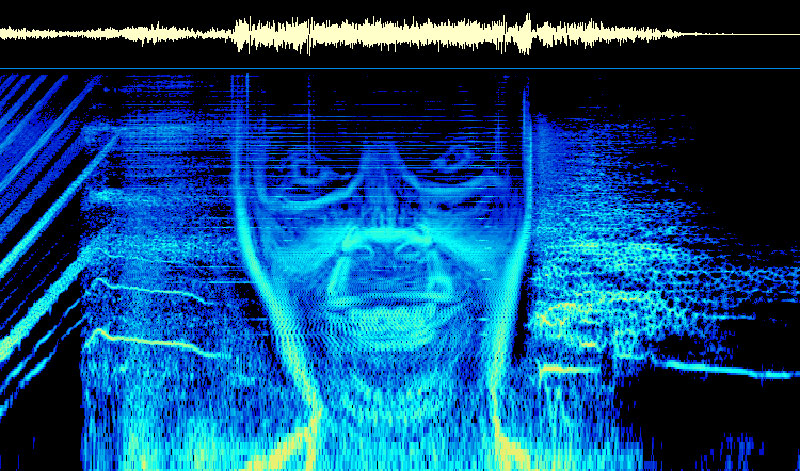
\includegraphics[width=\textwidth]{Background/equation-face.jpg}
    \caption{Spectrogram of $\Delta M_i^{-1} = - \alpha \sum_{n=1}^N D_i \left[ n \right] \left[ \sum_{j \in C \left[ i \right]}^{} F_{ji} \left[ n -1 \right] + Fext_i \left[ n^{-1} \right] \right]$~\cite{aphex-equation}}
\end{figure}

While this approach can theoretically convey all of the information held within the image, in practice, it is not feasible as a human visual aid. This method would require a human to perform a \ac{FFT} of the signal and re-construct the image in their head, and assumes that the auditory system has a sufficiently high bit-rate to receive all of the information, making the system unworkable --- little compression is performed. Additionally, the data is conveyed to the user in a column-by-column, time-multiplexed fashion, resulting in low temporal resolution.

\subsection{EyeMusic}
EyeMusic~\cite{abboud2014eyemusic} is fundamentally the same as vOICe, but with a different choice of sounds (instruments rather than sine waves), and additional image segmentation. It works by clustering the input image into red, green, white, blue and yellow components. Each colour is then assigned an instrument --- red is mapped to a reggae organ, green to a ``rapmans reed'' (a synthesised reeded instrument), white to a choir, blue to brass instruments and yellow to stringed instruments.

\begin{figure}[H]
    \centering
    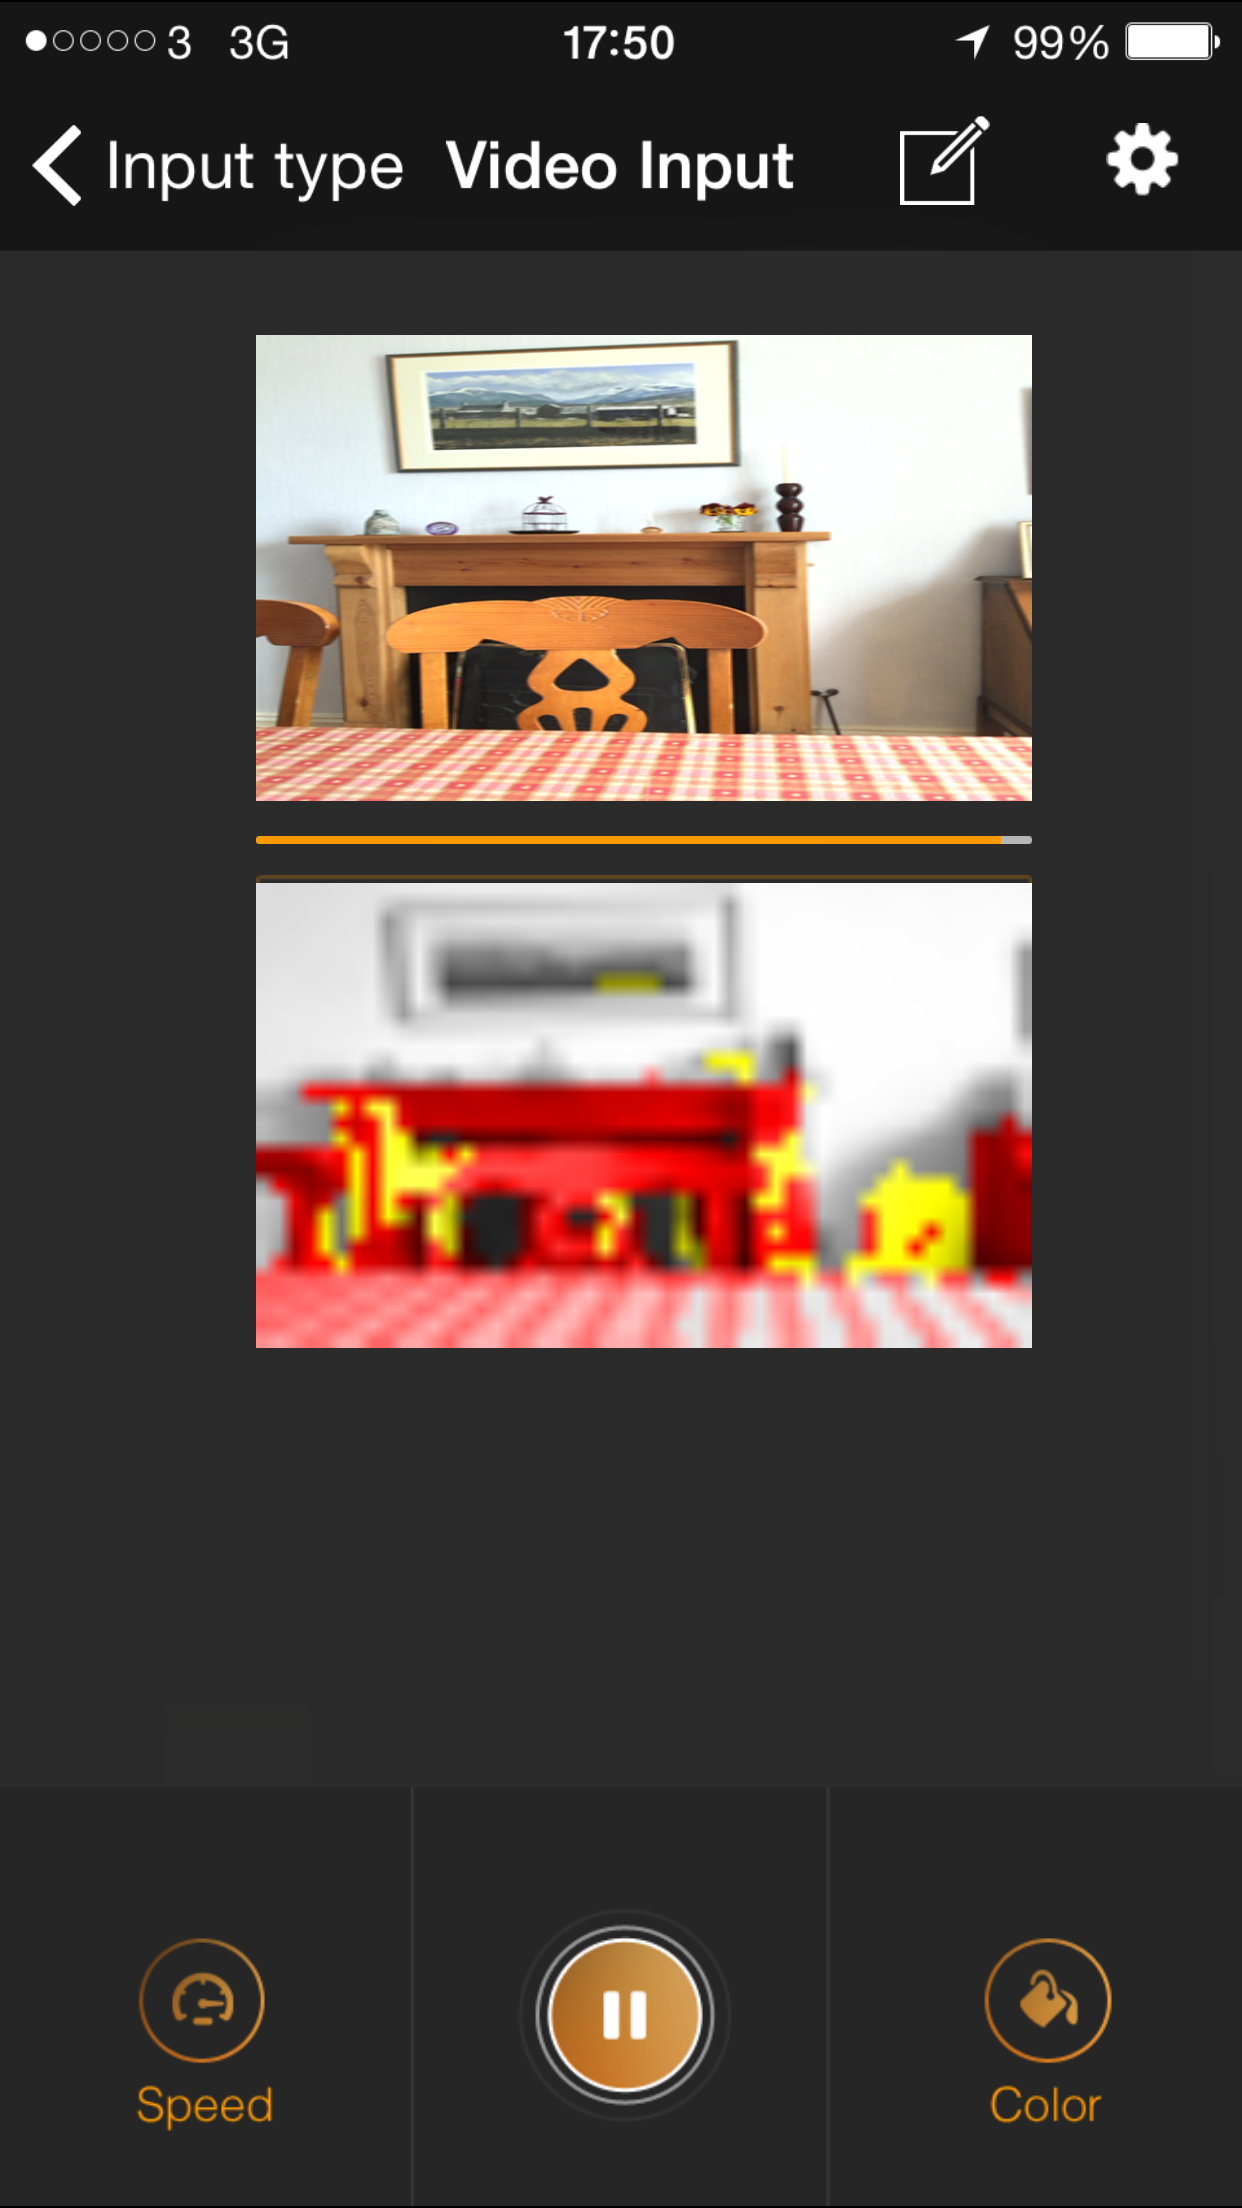
\includegraphics[width=0.4\textwidth]{Background/eyemusic.png}
    \caption{EyeMusic iOS Application}
\end{figure}

The resulting image is then scanned column-by-column, from left to right. A sound is then generated, with instrument varying according to pixel colour, pitch varying according to pixel position on the Y-axis, and volume according to the pixel luminance. The resulting sound is then played back for 50ms (by default), before moving on to the next column. 



\subsection{Virtual Acoustic Space}
\label{sec:vas}
A paper by Gonzalez-Mora, J.L. et al~\cite{vas} describes a method involving \ac{VAS}. \ac{VAS} works by simulating the sound that a user would hear if a point source at a particular angle and distance from the user was emitting a tone. For each frame, several points are placed --- the field of view of the camera is divided into a $17\times9$ grid, with a point inserted in each division. 

The system is not totally dissimilar to echo-location, but uses a simulated response from the objects, rather than relying on an ultrasonic echo.

\begin{figure}[H]
    \centering
    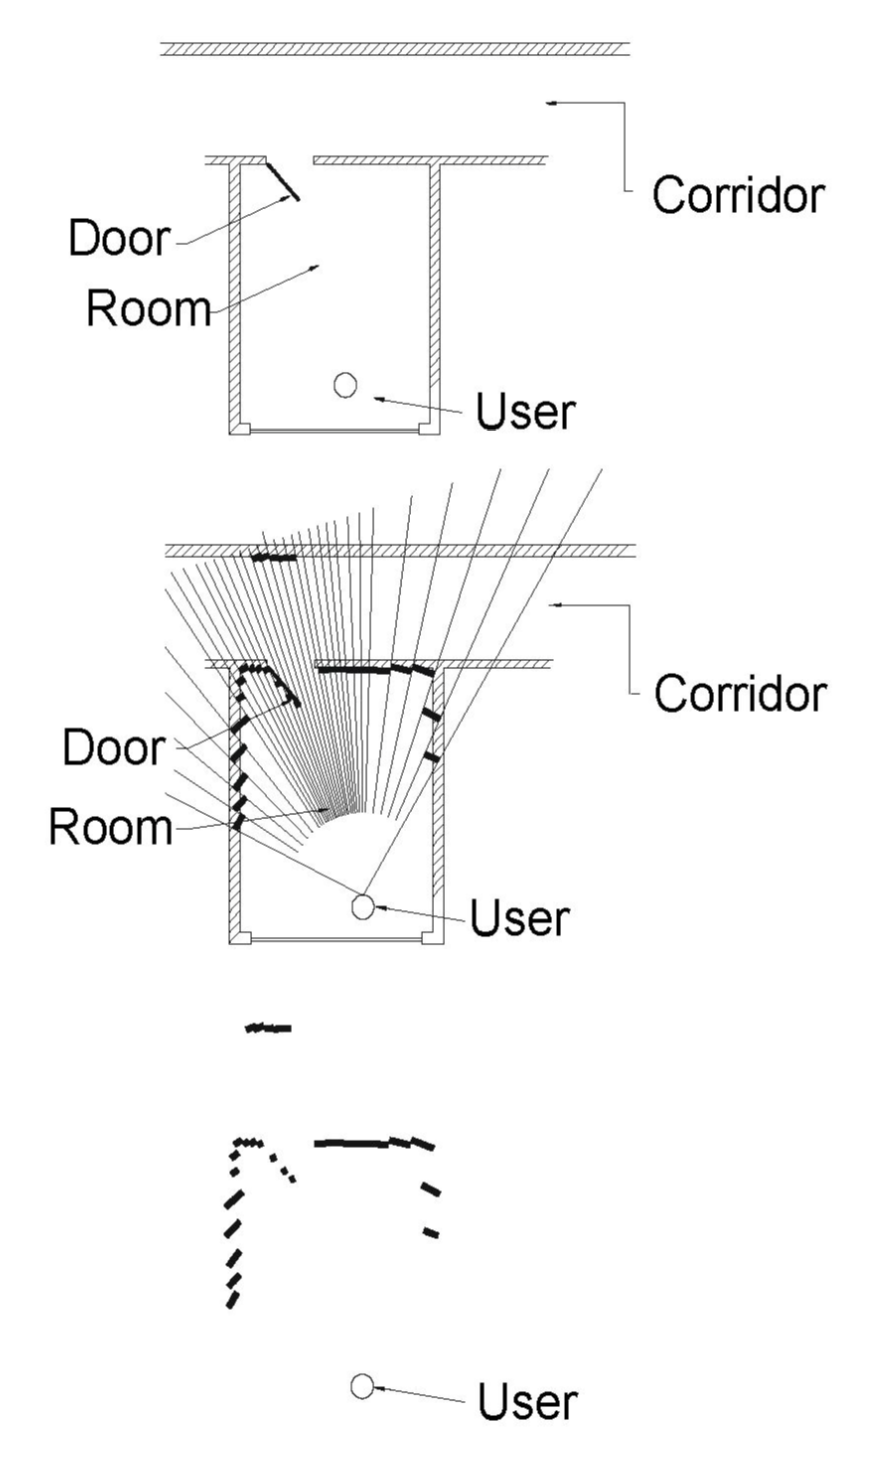
\includegraphics[width=0.5\textwidth]{Background/vas.png}
    \caption{Point placement with \ac{VAS}}
\end{figure}

The system described uses the \ac{HRTF} technique to apply filters to a tone. \ac{HRTF} works by modelling the effect the human body/head has on incoming audio. For instance, a tone emitted from a source to the left of a user has different properties when received on the left ear to the right ear; Higher frequencies will be attenuated more on the right ear, and there will be a slightly delay between the signal reaching each the right ear-drum compared to the left ear-drum. The \ac{HRTF} is applied to every point placed by the \ac{VAS} algorithm on both left and right channels. The modified tones (referred to as pips) are then played back in a random order. By inferring the position of each point based on it's acoustic properties, it has been shown that a trained user can navigate around a room.

\begin{figure}[H]
    \centering
    \includegraphics[width=0.25\textwidth]{Background/HRTF.png}
    \caption{Basis of HRTF technique~\cite{hrtf-diagram}}
\end{figure}

\subsection{TheVIBE}
``TheVIBE'' is a visuo-auditory sensory substitution system~\cite{thevibe}, which is similar in ways to the method discussed in section \ref{sec:vas}.

\begin{figure}[H]
    \centering
    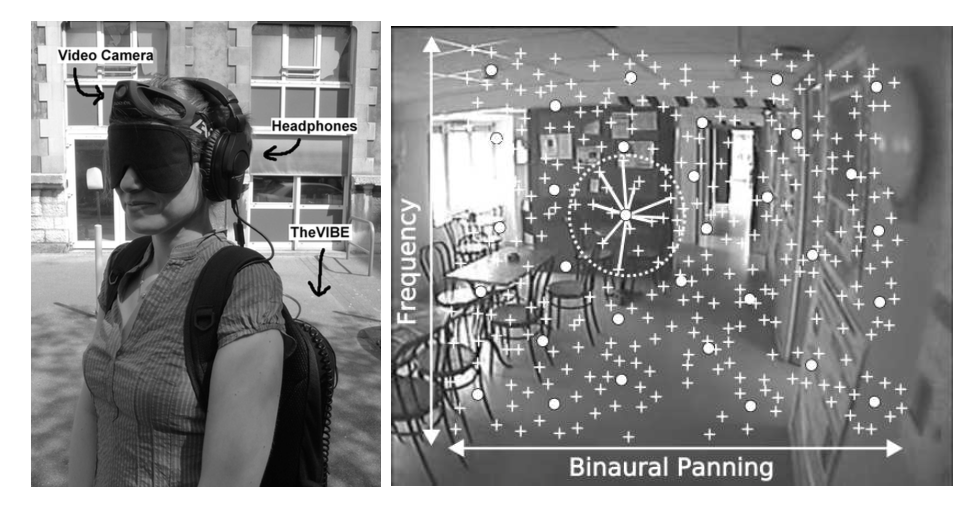
\includegraphics[width=\textwidth]{Background/thevibe.png}
    \caption{Visualisation of point spacing in TheVIBE}
\end{figure}

This paper describes a technique whereby points are assigned to ``receptive fields''. Each field has a static position, and is assigned loudness, determined by the Z-axis position of the points within the field. Unlike the method discussed in section \ref{sec:vas}, TheVIBE does not use a full \ac{HRTF} to convey field position; rather, it uses an inter-aural loudness difference (similar to stereo panning) to describe horizontal position, and tone frequency variation to describe vertical position.

\subsection{PSVA}
\ac{PSVA}~\cite{412057} works by dividing an input image (in this case, from a camera mounted on the users head) into a grid and assigning a frequency to each pixel, according to the formula:

\begin{equation}
    f_{n} = f_{c} \times 2^{n/128}
\end{equation}

where $f_{c}$ is a central frequency, around which pixel frequencies are based, and $n$ is the pixel number. 

Additionally, edge detection is performed (through Laplacian of Gaussian) in order to more effectively mimic the processing normally done by the human visual system.

The phase of the sound being generated by each pixel depends on it's horizontal position, with the amplitude of the sound depending on the grey-level intensity of the pixel. The tones are then played back simultaneously (having been generated by an inverse Fourier transformation) and in real-time --- the system was prototyped on an \ac{FPGA}, presumably due to the limited speed of normal processors at the time of the paper's publication (1993). 

With this system, the varying sensitivity of the human eye is accounted for by increasing the size of the pixels at the periphery of the image, resulting in an increased central resolution.

\subsection{Summary of disadvantages of existing solutions}
The existing solutions to the problem of video to audio conversion all suffer from a similar problem --- information overload, and training time (due in part to neuroplasticity).

With the exception of PSVA, these solutions are also afflicted with a low temporal resolution, due to the time-multiplexing mode of operation. There is also little prioritisation of information being conveyed to the user, beyond varying the size of the receptive field being performed with PSVA.


\chapter{Approach}
\section{Image Segmentation}
Although the primary deliverable of the project was not to invent a new image segmentation algorithm, the method of image segmentation was an important choice.

It was decided that a depth-sensing camera~\cite{xtion} would be used in order to assist with region extraction. Rather than relying solely on RGB data and difference in colour to extract objects from the video footage, depth data would also be considered. This choice was made, as object-segmentation was desired --- if a white cup was placed on a white table, traditional colour-based segmentation algorithms may struggle to differentiate between the object and the surfact on which the object was sitting.

As majority of image segmentation algorithm implmentations consider only colour information for segmentation; it was not possible to use an off-the-shelf MATLAB module to complete this task. After reviewing publications on segmentation using both depth and RGB data, a few different approaches were trialled.

\subsection{Standard Deviation}
As an intial experiment, I attempted to highlight ``interesting'' sections of the image. This was accomplished by using a sliding window over the RGB image, calculating the standard deviation of the pixels in the window. The resulting image was then thresholded and used on a mask on the orignal image,

This method was quite succesful - the resulting image only contained objects that stood out on the input image.

\begin{figure}[H]
    \centering
    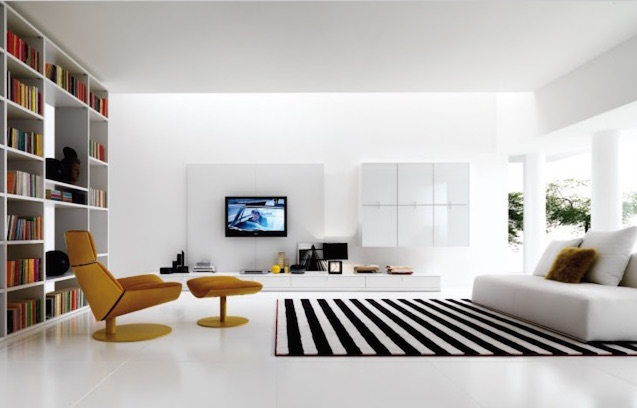
\includegraphics[width=0.6\textwidth]{Segmentation/sd-input.jpg}
    \caption{Input Image}
\end{figure}

\begin{figure}[H]
   \centering
   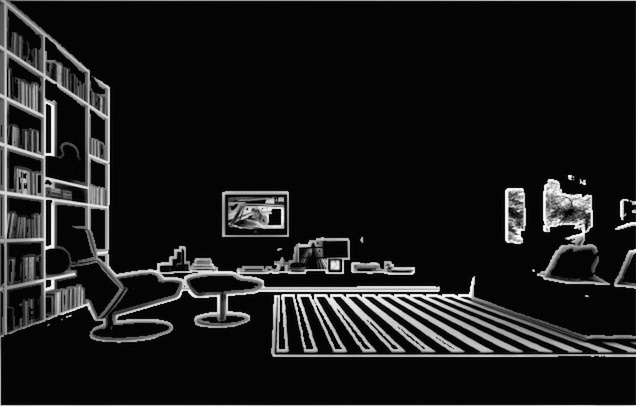
\includegraphics[width=0.6\textwidth]{Segmentation/sd-output.jpg}
   \caption{Standard Deviation Results}

\end{figure}

The main issue with this approach was that Depth Information was not used - cases where objects had little RGB contrast would not be picked out. 

\subsection{K-Means with 4 channels}
One approach was to use a standard K-Means image segmentation algorithm~\cite{kmeans-matlab}, with an additional channel added, representing depth. 

\begin{figure}[H]
    \centering
    \begin{subfigure}[b]{0.45\textwidth}
        \centering
        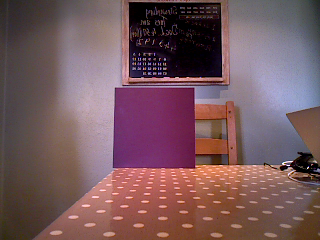
\includegraphics[width=\textwidth]{Segmentation/squarergb-10.png}
        \caption{Input RGB Image}
    \end{subfigure}
    \hfill
    \begin{subfigure}[b]{0.45\textwidth}
        \centering
        
\includegraphics[width=\textwidth]{Segmentation/squaredepth-10.png}
        \caption{Input Depth Map}
    \end{subfigure}
\end{figure}

\begin{figure}[H]
    \centering
    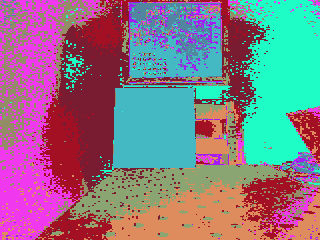
\includegraphics[width=0.4\textwidth]{Segmentation/kmeans-rgb-10seg-im9.png}
    \caption{RGB-only K-Means segmentation}
\end{figure}

\begin{figure}[H]
    \centering
    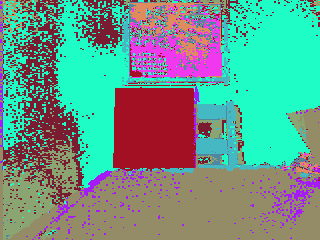
\includegraphics[width=0.4\textwidth]{Segmentation/kmeans-rgb-depth-10seg-im9.png}
    \caption{RGBD K-means segmentation}
\end{figure}

This was fairly succesful, however was very vulnerable to noise - only images acquired in environments with perfect lighting provided good segmentation results. 

These results were fairly good - the addition of the depth channel resulted in a smoother segmentation. However, using raw images from the camera for segmentation resulted in a fairly noisy image. Applying a gaussian blur to the image (\diameter = 5, \sigma = 2) removed some of the noise, at the expense of sharpness in the image.

\begin{figure}[H]
    \centering
    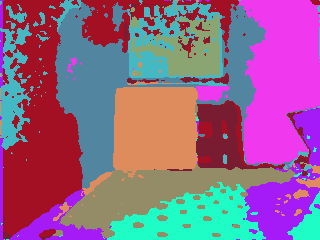
\includegraphics[width=0.4\textwidth]{Segmentation/rgb-depth-kmeans-blurred-10.png}
    \caption{Segmentation of blurred RGBD image}
\end{figure}

\subsection{K-Nearest Neighbour}

\subsection{Channel Swapping}
As mentioned, most segmentation algorithms support only RGB data. With this in mind, another approach taken was to remove a colour channel from the RGB image, and swap it with the depth image. This was quite sucessful --- the resulting segmentation was more accurate than either RGB or Depth alone.

\subsection{Graph Cuts}
Attempts were made to use the Graph Cuts algoritm [REF] in order to segment the video and depth data. However, it became apparent that this approach was taking orders of magnitude longer than we could reasonably spend processing each frame; we wanted the system to run as close to real-time as possible.

\section{Feature Extraction}

\subsection{Basis Shapes}

\subsubsection{Zernike Moments}
Zernike Moments ---ref--- are a set of orthogonal moments ---EXPAND---. Due to their orthogonality, it is possible for a computer to compress an image or shape very efficiently using Zernike Moments. 

With this in mind, I attempted to express the extracted shape in terms of Zernike Moments --- the theory being that given the Zernike moments, a human may be able to re-construct the image mentally.

By assigning a harmonic to each Zernike moment, and varying the amplitude of each harmonic according to the moment value, a tone was generated. I then proceeded to pass various shapes into the algorithm, listening to the tone.

Although the tone varied with each shape, it was not possible to identify individual shapes using this system --- it was unclear how a change in the amplitude of a particular harmonic corresponded to changes in shape. 


\clearpage
\section*{List of Acronyms}
\begin{acronym}
\acro{WHO}{World Health Organisation}
\acro{IR}{Infra-red}
\acro{RGB-D}{Red, Green, Blue and Depth}
\acro{RGB}{Red, Green and Blue}
\acro{FFT}{Fast-Fourier transform}
\acro{VAS}{Virtual Acoustic Space}
\acro{HRTF}{Head-related transfer function}
\acro{JVM}{Java Virtual Machine}
\acro{FOV}{Field of View}
\acro{EFT}{Elliptic Fourier Transform}
\end{acronym}



\clearpage
\printbibliography


\end{document}
